\chapter{Ausblick} \index{Ausblick}

In dieser Arbeit wurde nun die Basis f�r einen multifunktionelles Ger�t zur Timing-, Protokoll-, Logik- und Eventanalyse von digitalen Signalen geschaffen.

Um nun aus dieser Plattform ein voll funktionsf�higes Ger�t zu erstellen, m�ssen noch folgende Arbeiten erledigt werden.

\begin{description} 
 \item[USB-Schnittstelle:] F�r die in Kapitel \ref{USB-Schnittstelle} erl�uterte USB-Schnittstelle muss noch die Konfiguration des Logibausteins fertig implementiert werden. F�r Windows-Systeme sollte noch eine .inf-Datei erzeugt werden, um eine problemlose Integration zu erm�glichen.
 \item[Mikrocontroller-Software:] Hier muss die Kommunikationsschnittstelle mit dem CPLD sowie die Aufbereitung der Messdaten implementiert werden. Siehe Kapitel \ref{Mikrocontroller_Software}.
 \item[VHDL-Design:] Das in Kapitel \ref{VHDL-Design} beschriebene VHDL-Design kann auf Basis der bereits erzeugten Quartus-II-Projektdateien implementiert werden.
 \item[PC-Software] Es k�nnte auch eine grafische Bedieneroberfl�che (GUI) erzeugt werden. Dadurch l�sst sich der Analysator nicht nur �ber ein Text-Terminal, sondern auch komfortabel mit der Maus bedienen. Hier k�nnte auch die graphische Anzeige der Messwerte mit integriert werden.
 \end{description}

Diese Arbeiten k�nnen nun, zum Beispiel durch eine Projektkruppe im Rahmen der technischen Projektarbeit oder in einer Abschlussarbeit durchgef�hrt werden.

Durch die sehr flexible Kombination aus Mikrocontroller mit USB-Schnittstelle, Logikbaustein und Speicher, sind allerdings auch viele andere Projekte auf dieser Hardwarebasis denkbar.

\chapter{Anhang}

\section{Schaltplan und Platinenlayout}

\begin{figure}[ht]
	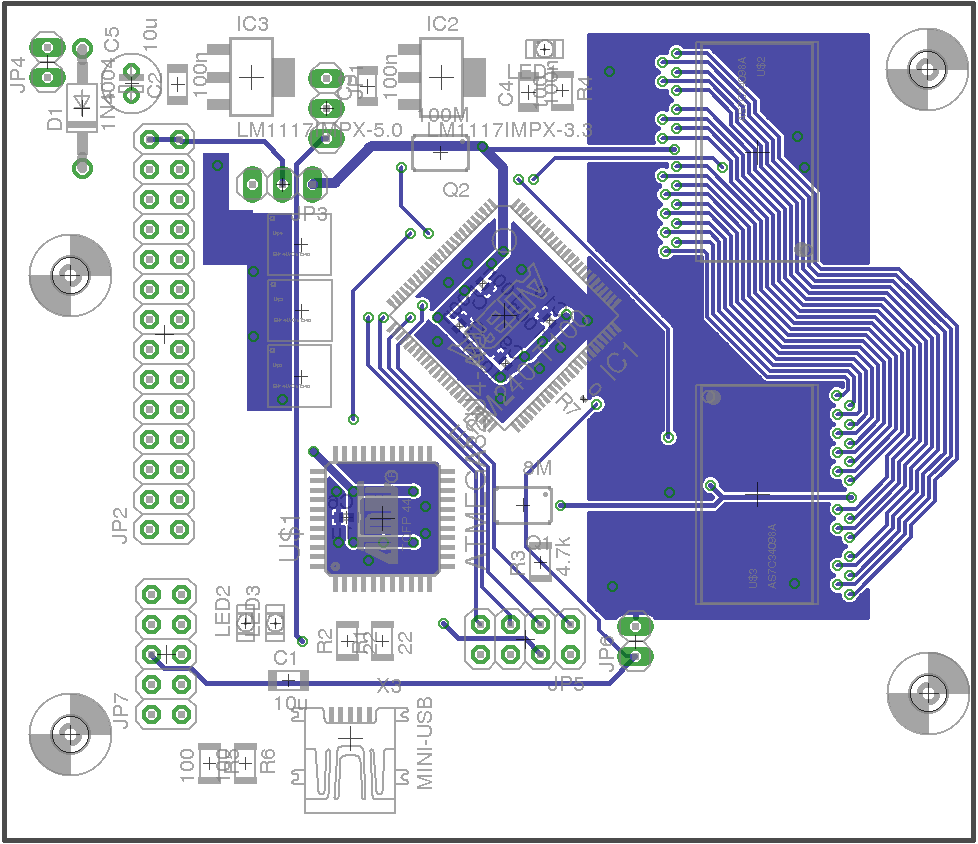
\includegraphics[width=1.0\textwidth]{images/Platine_bot.png}\\
	\rule{\linewidth}{0.5pt}
	\caption{Platinenlayout, Unterseite}
\end{figure}

\begin{figure}[ht]
	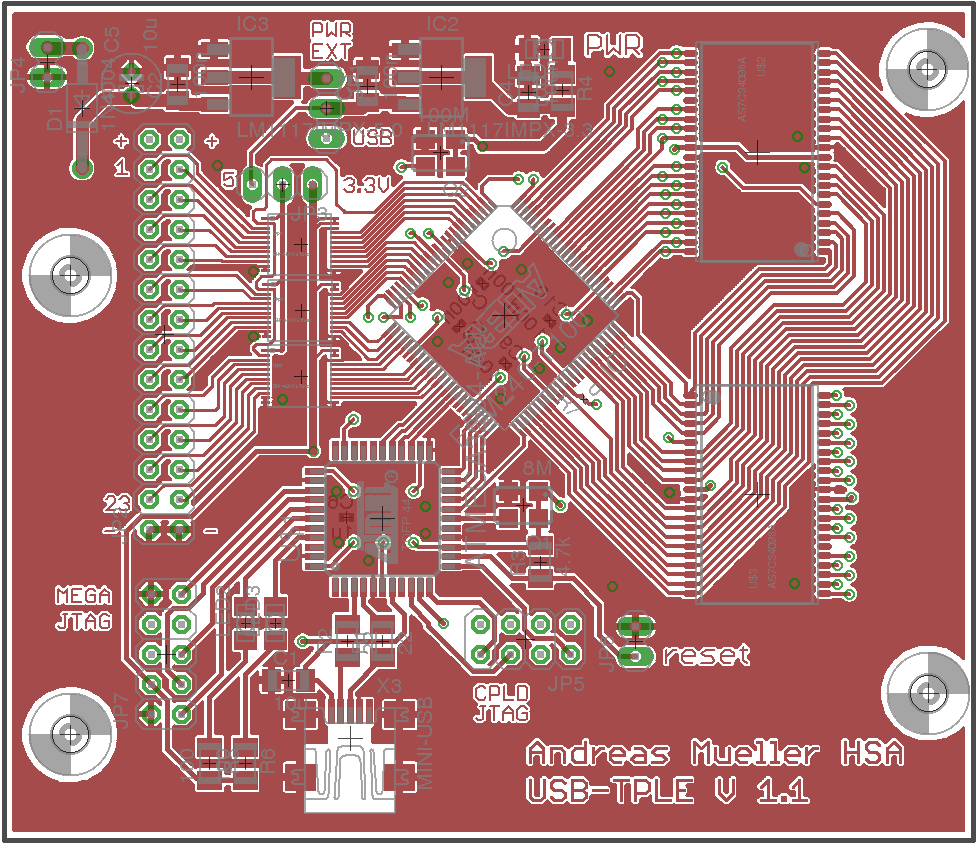
\includegraphics[width=1.0\textwidth]{images/Platine_top.png}\\
	\rule{\linewidth}{0.5pt}
	\caption{Platinenlayout, Oberseite}
\end{figure}

\begin{landscape}
%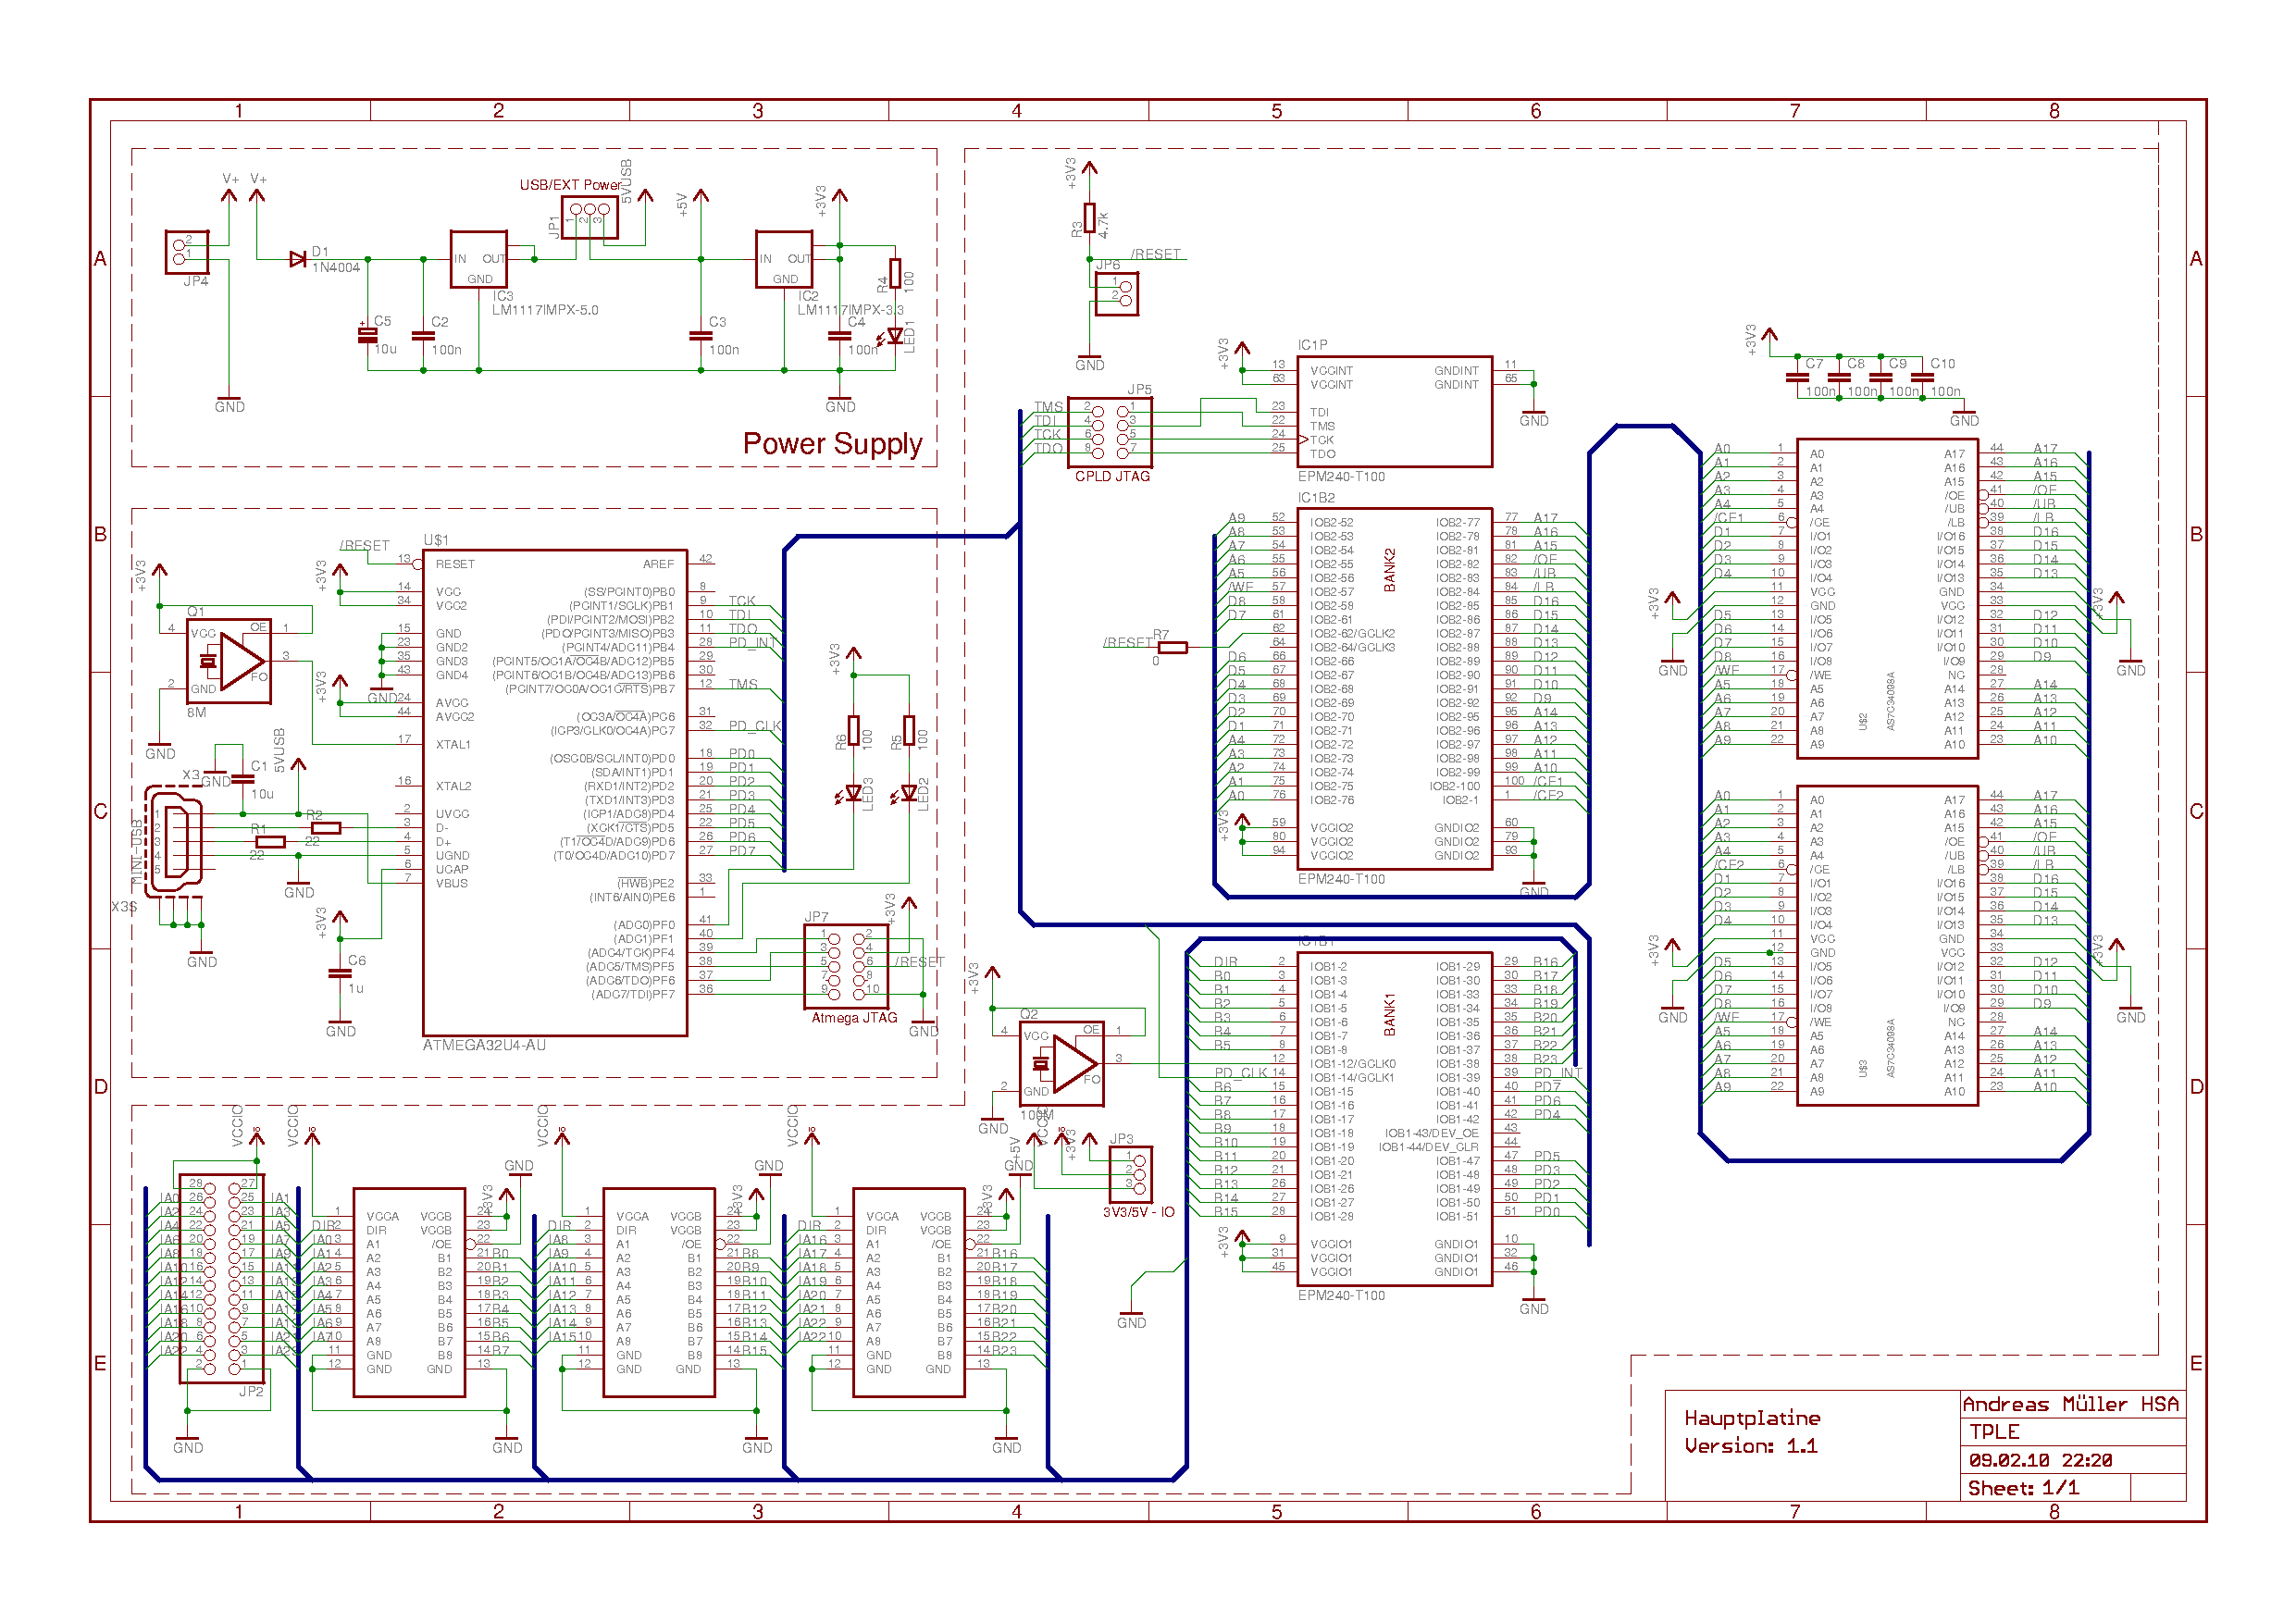
\includepdf{images/main_cirquit_v1_1.pdf}
%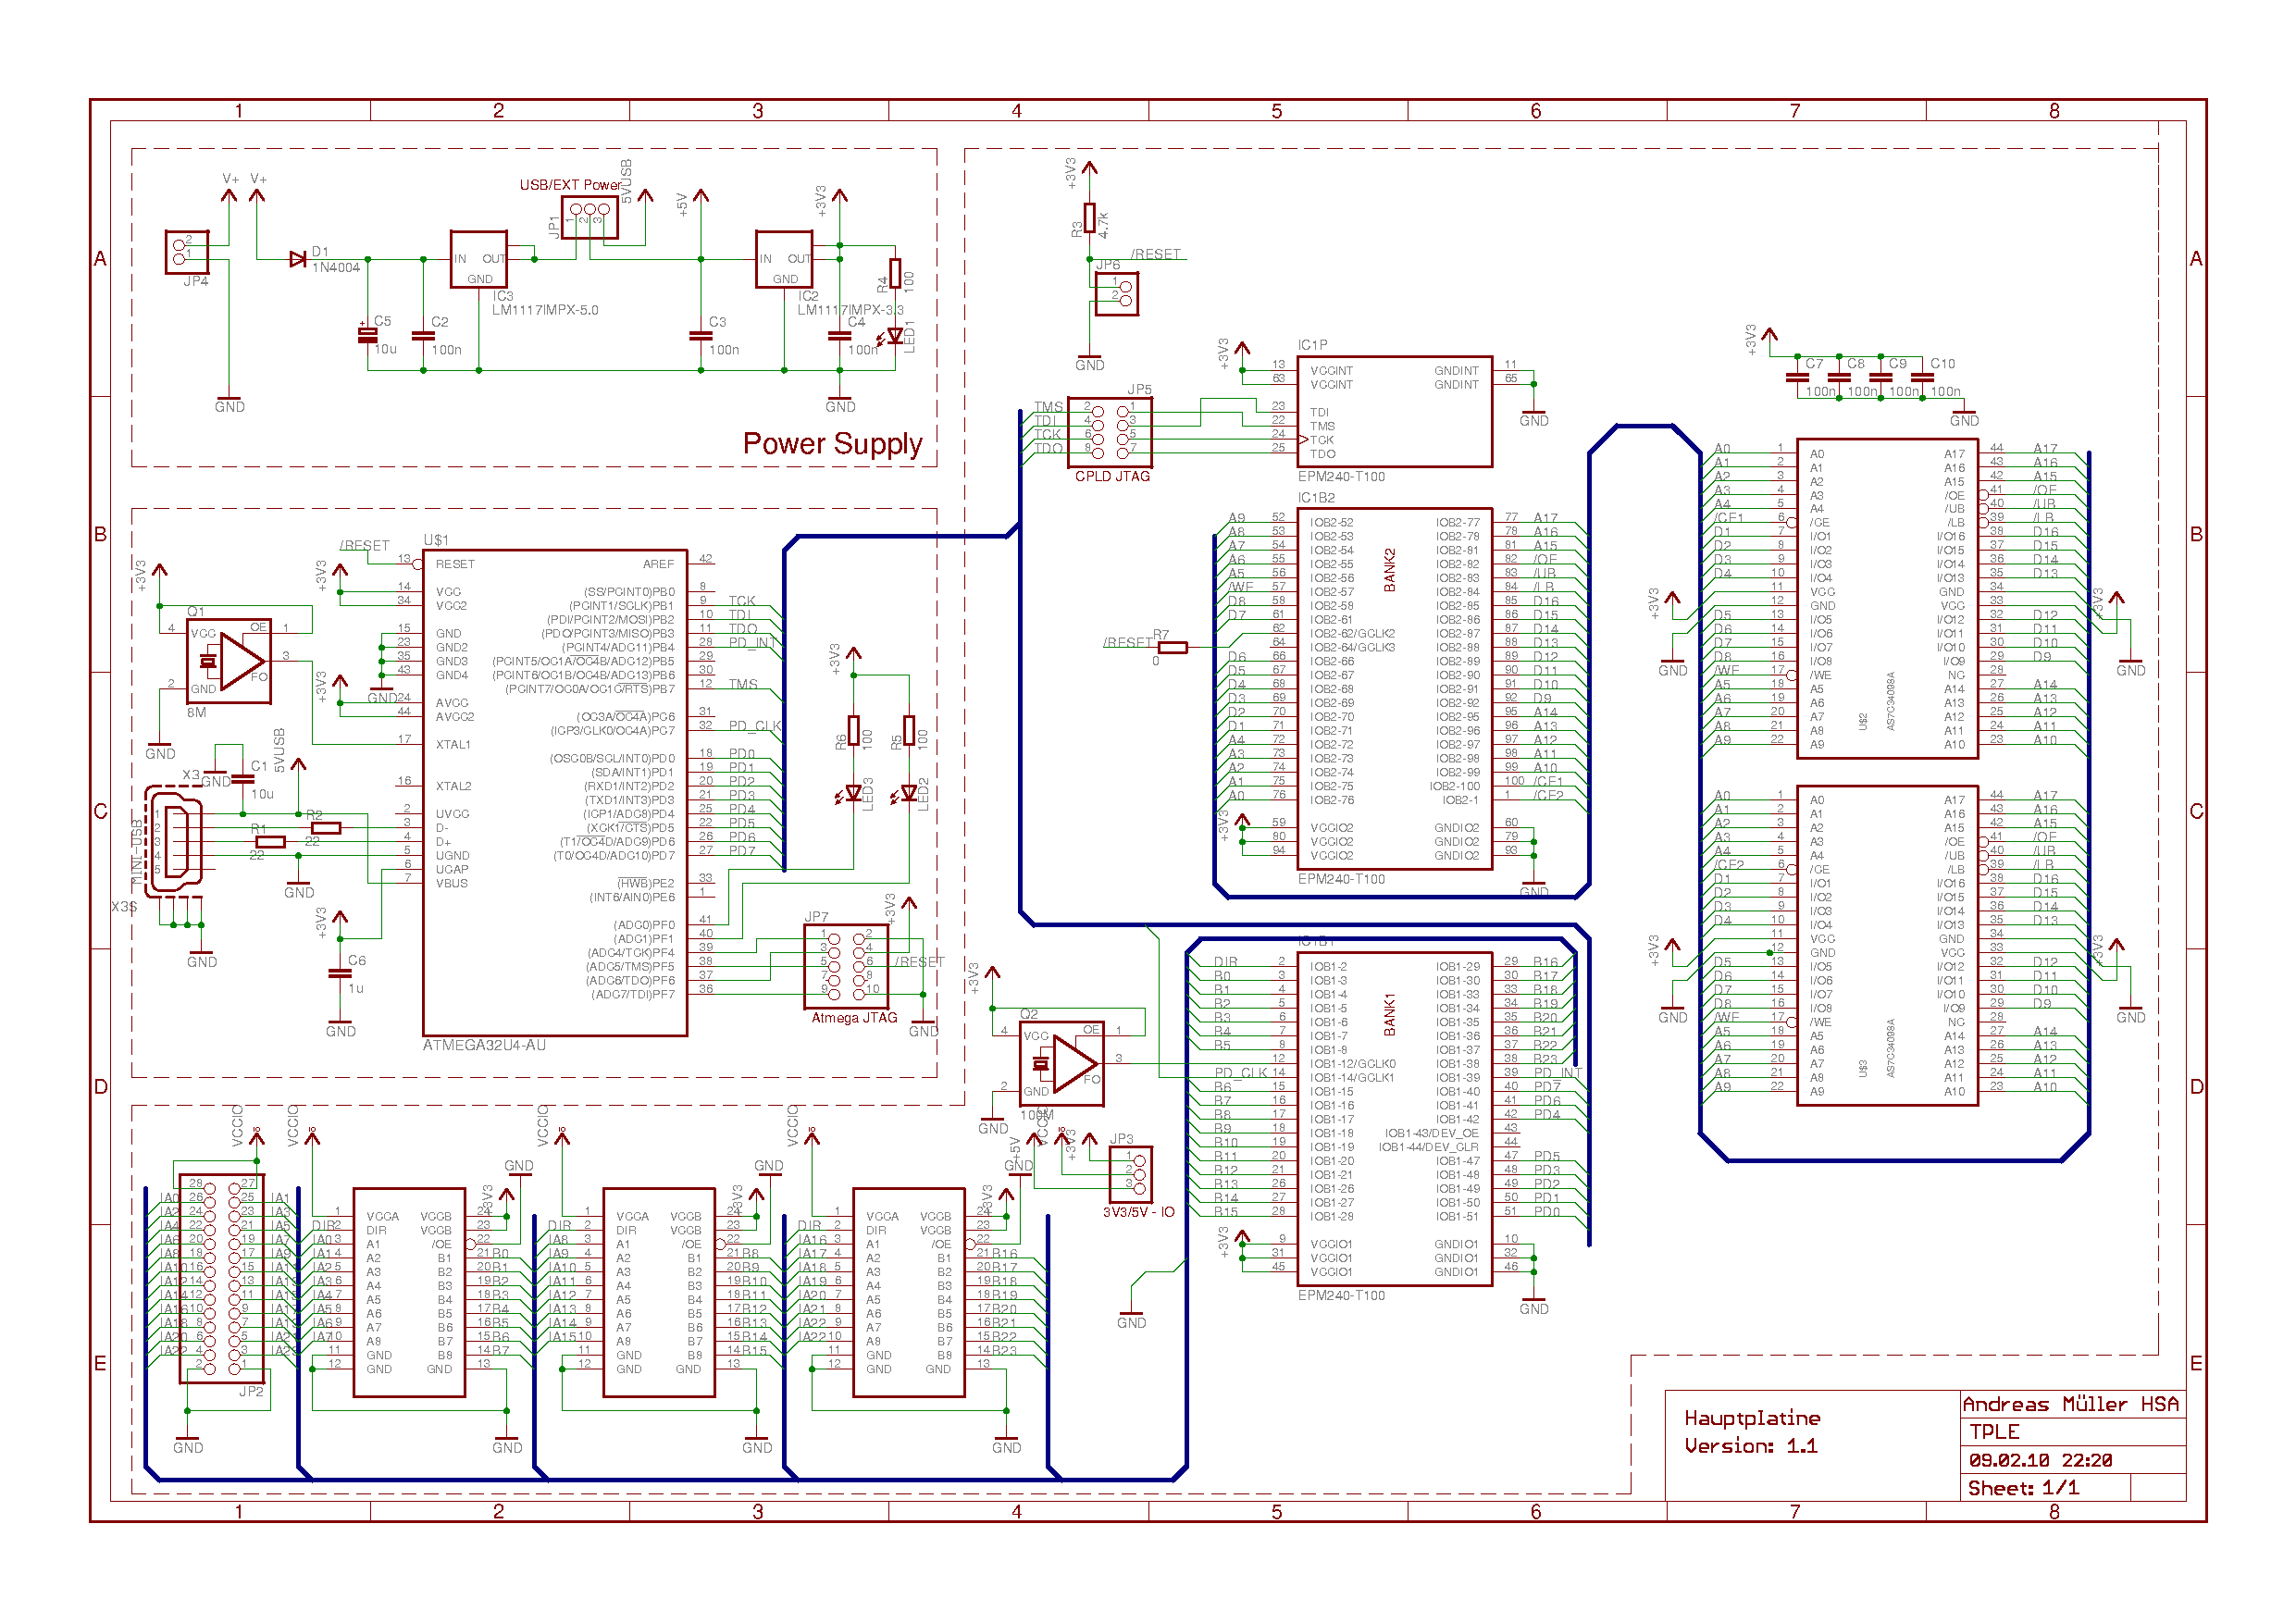
\includegraphics{images/main_cirquit_v1_1.pdf}
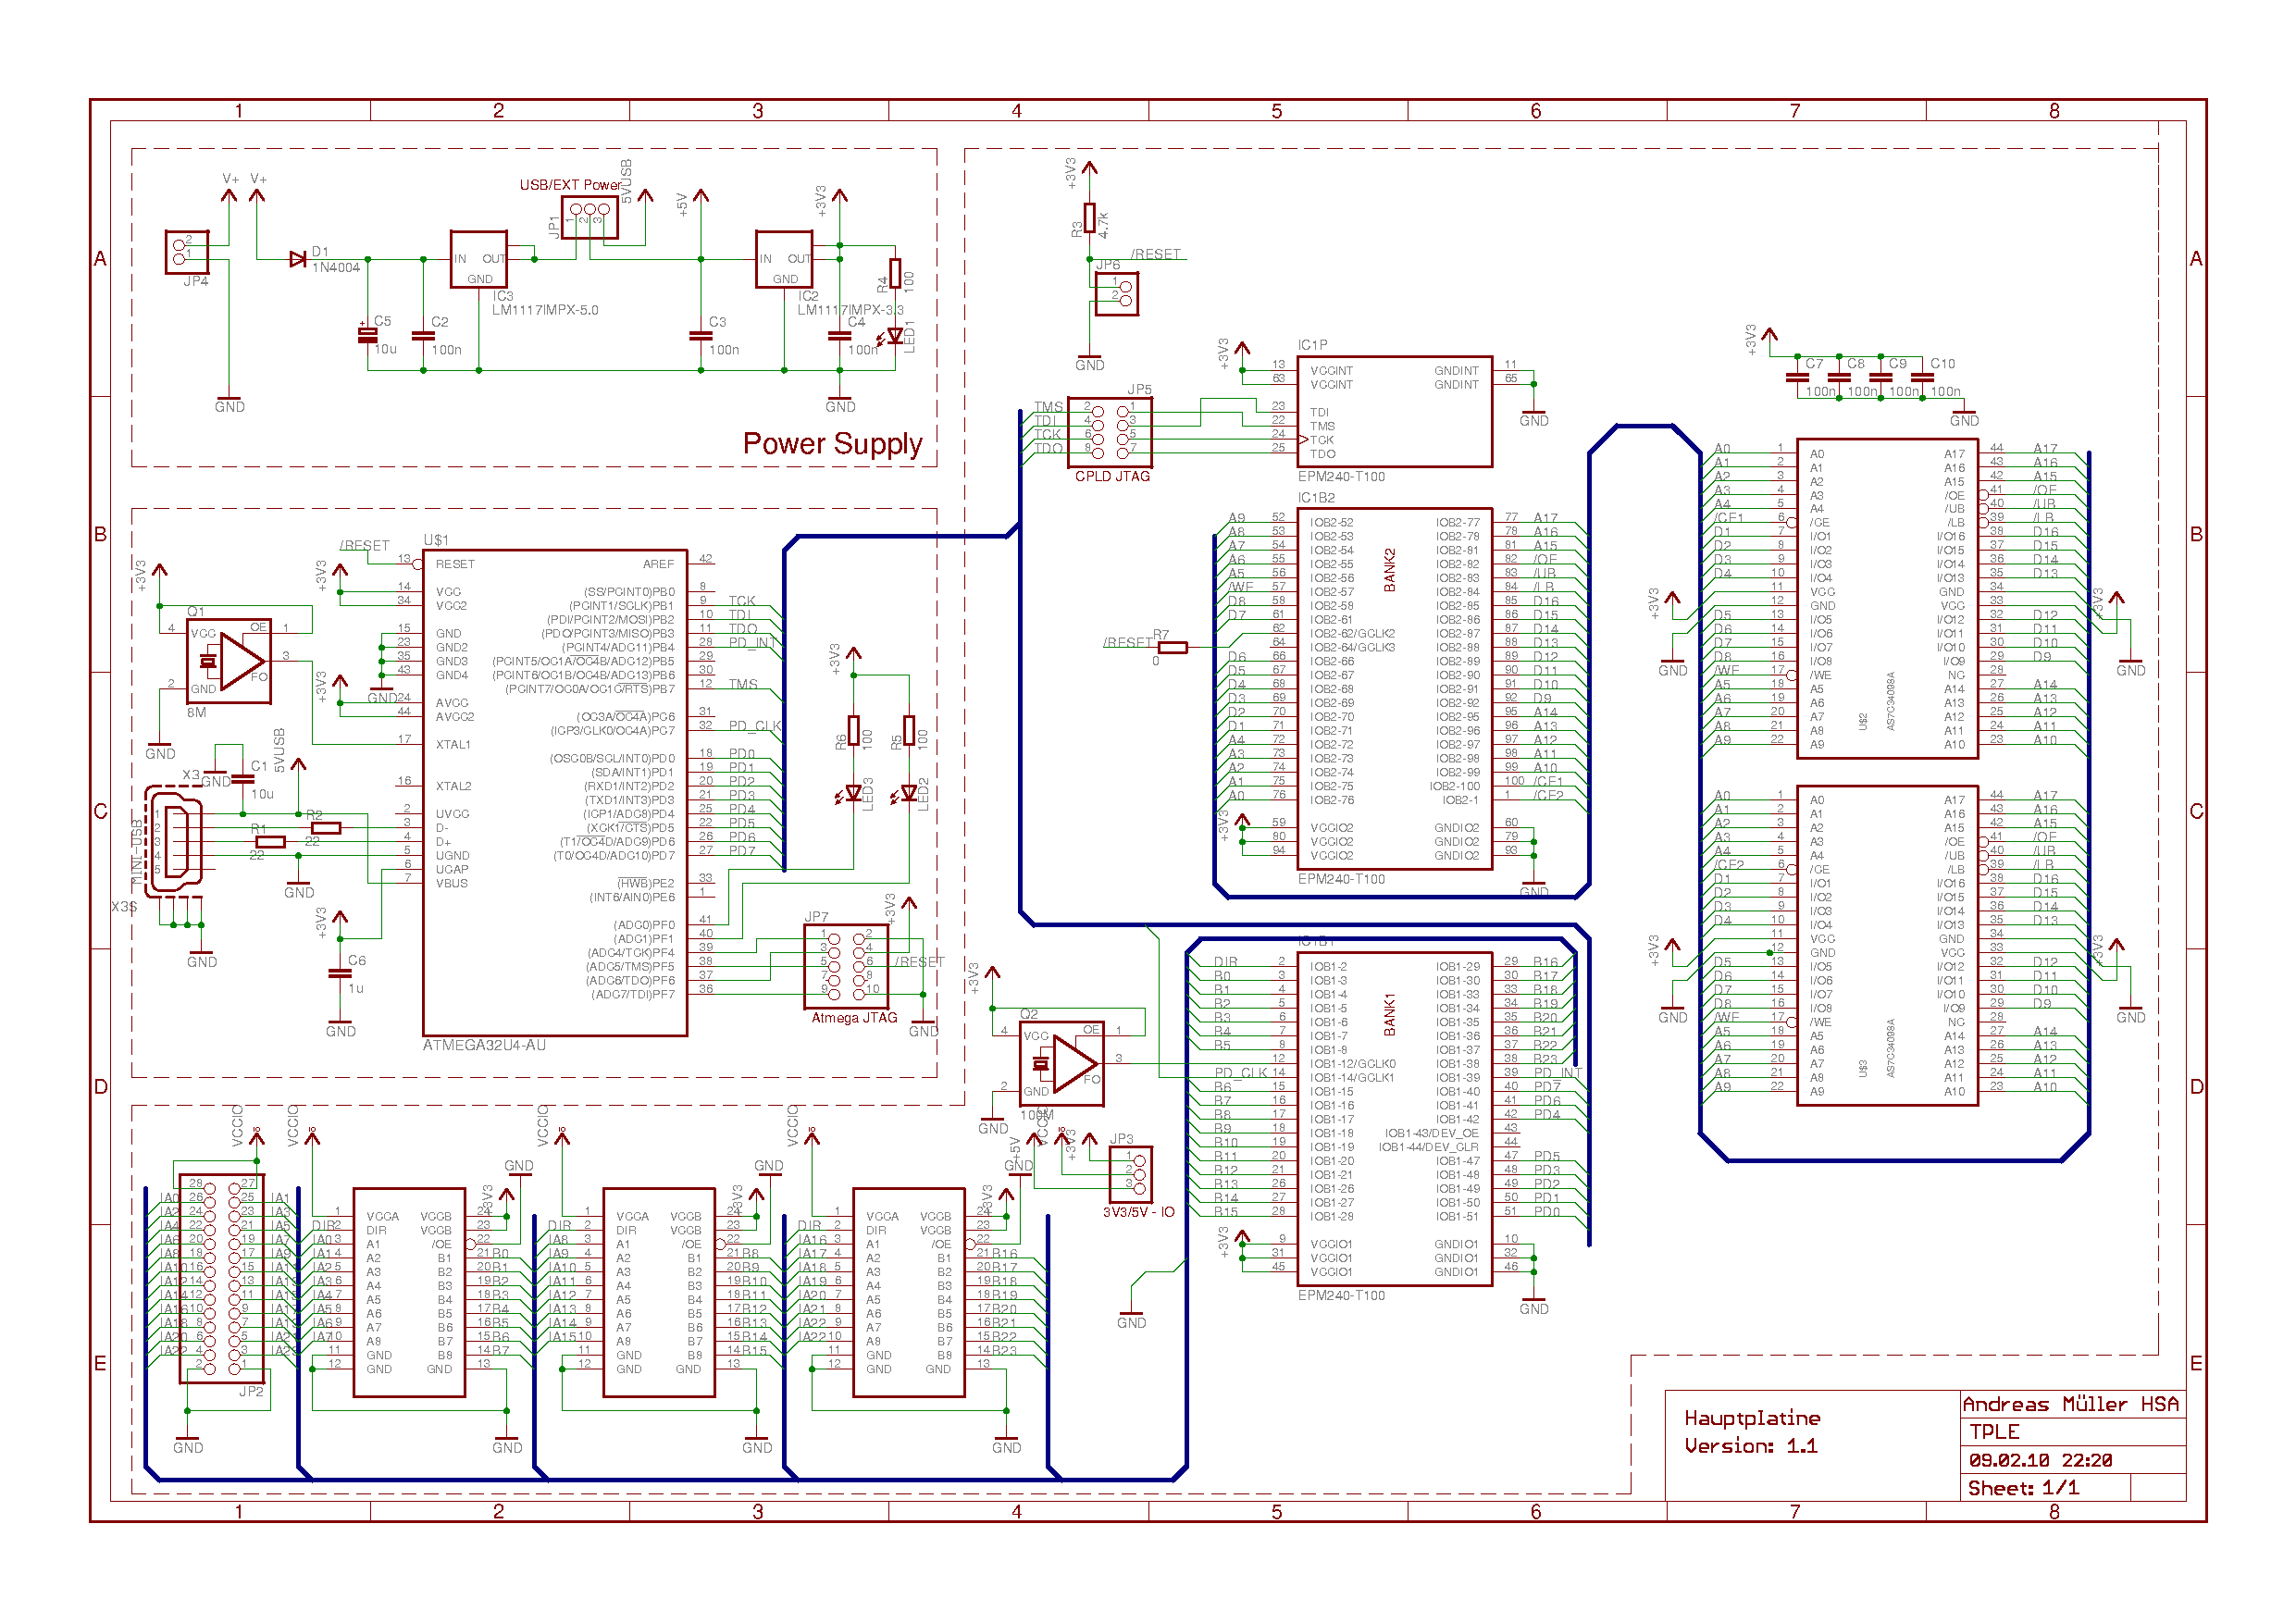
\includegraphics[width=1.4\textwidth]{images/main_cirquit_v1_1.pdf}
\end{landscape}

\section{Bauteile}

\begin{table}[h] 
\begin{tabular}{|l|l|l|l|l|}
\hline
Menge	& Wert		& Bezeichnung		& Bauteilname		& Farnell Bestellnummer \\
\hline \hline
2	& 1X2		& PINHEAD		& JP4, JP6		& ------- \\
2	& 1X3		& PINHEAD		& JP1, JP3 		& ------- \\
1 	& 2X4		& PINHEAD		& JP5			& ------- \\
1	& 2X5		& PINHEAD		& JP7			& ------- \\
1	& 2X14		& PINHEAD		& JP2			& ------- \\
1	& 		& MINI-USB		& X3			& 1558179 \\
2	& 22		& R3216			& R1, R2		& 1577421 \\
1	& 4.7k		& R3216			& R3			& 1717749 \\
3	& 100		& R3216			& R4, R5, R6		& 1717738 \\
1	& 0		& R0201			& R7			& ------- \\
1	& 10u		& C3216			& C1			& 1432339 \\
3	& 100n		& C1206			& C2, C3, C4		& 1759312 \\
1	& 10u		& CPOL2-5		& C5			& ------- \\
1	& 1u		& C0402			& C6			& 1611915 \\
4	& 100n		& C0402			& C7, C8, C9, C10	& 1611916 \\
1	& 1N4004	& Diode			& D1			& 9556109 \\
1	& 8M		& Oszilator		& Q1			& ------- \\
1	& 100M		& Oszilator		& Q2			& 1538960 \\
3	& RED		& LED1206		& LED1, LED2, LED3	& 1318261 \\
1	& ATMEGA32U4-AU	& Microcontroller	& U\$1			& ------- \\
2 	& AS7C34098A	& Memory		& U\$2, U\$3		& 1562920 \\
1	& EPM240-T100	& Altera CPLD		& IC1			& 1453502 \\
1	& LM1117IMPX-3.3 & Regulator		& IC2			& 1652313 \\
1     	& LM1117IMPX-5.0 & Regulator		& IC3			& 1652314 \\
3	& SN74LVC8T245	& BUS-Driver		& U\$4, U\$5, U\$6	& 1236406 \\
\hline
\end{tabular}
\caption{Liste aller n�tigen Bauteile mit Bestellnummern (Falls vorhanden)}
\label{tab:Bauteile}
\end{table}

\newpage

\section{Inhaltsverzeichnis Datentr�ger}

\begin{table}[h] 
\begin{tabular}{|l|l|}
\hline
Verzeichnis						& Beschreibung	\\
\hline \hline
./							& Wurzelverzeichnis \\
./PLD\_Firmware						& Firmware Logikbaustein \\
./PLD\_Firmware/src					& VHDL-Quellcode \\
./PLD\_Firmware/Quartus\_project			& Quartus-II Projektdateien \\
./Microcontroller\_Firmware				& Firmware Mikrocontroller \\
./Microcontroller\_Firmware/LUFA\_Based			& Quellcode Verzeichnis f�r Lufa-Basierenden Quellcode \\
./Microcontroller\_Firmware/LUFA\_Based/estick\_firmware & Estick-JTAG Adapter \\
./Microcontroller\_Firmware/LUFA\_Based/DualSerial	& Duale virtuelle serielle Schnittstelle \\
./Microcontroller\_Firmware/Atmel\_Based		& Quellcode Verzeichnis f�r Lufa-Basierenden Quellcode \\
./Microcontroller\_Firmware/Atmel\_Based/USB\_JTAG\_UART& Jam-Player basierender JTAG-Adapter \\
./Microcontroller\_Firmware/Atmel\_Based/Bootloader	& Atmel Bootloader \\
./Datasheets						& Datenbl�tter \\
./Hardware						& Verzeichnis f�r Schaltpl�ne und Boardlayouts \\
./Hardware/V1.1						& Hardware Revision 1.1 \\
./Hardware/eagle\_lib					& Nicht-Stadard Eagle Bibliotheken \\
./Hardware/V1.0						& Hardware Revision 1.0 \\
./Documentation						& Dokumentation \\
./PC\_Software						& PC-Software \\
./PC\_Software/urjtag-0.10				& UrJTAG \\
./PC\_Software/DFU\_programmer				& Bootloader PC-Software \\
./PC\_Software/USB\_STAPL\_Player			& Software zur CPLD-Konfiguration \\
\hline
\end{tabular}
\caption{Inhaltsverzeichnis Datentr�ger}
\label{tab:Datentraeger}
\end{table}

\listoffigures

% Literaturverzeichnis soll im Inhaltsverzeichnis auftauchen
\addcontentsline{toc}{section}{Literatruverzeichnis}

\begin{thebibliography}{------} \label{Literaturverzeichnis}

\bibitem[Hoffm02]{Hoffm02}
	J. Hoffmann, W. Trentmannm:
	{\em Praxis der PC-Messtechnik}.
	Hanser, 2002 \\
	ISBN 3-446-21708-8 \\

\bibitem[Schwe97]{Schwe97}
	H. Schwetlick:
	{\em PC-Messtechnik}.
	Vieweg, 1997 \\
	ISBN 3-528-04948-4 \\

\bibitem[Kaink00]{Kaink00}
	B. Kainka:
	{\em Messen, Steuern und Regeln mit USB}.
	Franzis Verlag, 2000 \\
	ISBN 3-7723-5874-8 \\

\bibitem[Atmel01]{Atmel01}
	Atmel:
	{\em Atmega32-U4 Datasheet} \\
	\url{http://www.atmel.com/dyn/resources/prod\_documents/doc7766.pdf}\\
	Rev. Juli 2008 \\

\bibitem[Alter01]{Alter01}
	Altera:
	{\em MAX II Device Handbook} \\
	\url{http://www.altera.com/literature/hb/max2/max2\_mii5v1.pdf}\\
	Rev. August 2009 \\

\bibitem[Xilin01]{Xilin01}
	Xilinx:
	{\em Coolrunner II Data Sheet} \\
	\url{http://www.xilinx.com/support/documentation/data\_sheets/ds090.pdf}\\
	Rev. September 2008 \\

\bibitem[Texas01]{Texas01}
	Texas Instruments:
	{\em SN74LVC8T245 Data Sheet} \\
	\url{http://www.ti.com/lit/gpn/sn74lvc8t245}\\
	Rev. Juni 2005 \\ 

\bibitem[Allia01]{Allia01}
	Alliance Memory:
	{\em AS7C34098A Data Sheet} \\
	\url{http://www.alliancememory.com/pdf/sram/fa/as7c34098a\_v2.1.pdf}\\
	Rev. August 2004 \\

\bibitem[Atmel02]{Atmel02}
	Atmel:
	{\em AVE329: USB Firmware Archtecture} \\
	\url{http://www.atmel.com/dyn/resources/prod\_documents/doc7703.pdf}\\
	Rev. Februar 2006 \\

\bibitem[Lufa01]{Lufa01}
	Lufa Homepage \\
	\url{http://www.fourwalledcubicle.com/index.php}\\
	Rev. 13. Mai 2010 \\

\bibitem[Alter02]{Alter02}
	Altera:
	{\em Using Jam STAPL for ISP via an Embedded Processor} \\
	\url{http://www.altera.com/literature/hb/max2/max2\_mii51015.pdf}\\
	Rev. Oktober 2008 \\

\bibitem[Khirm01]{Khirm01}
	Stas Khirman:
	{\em JTAG FAQ} \\
	\url{http://hri.sourceforge.net/tools/jtag\_faq\_org.html}\\
	Rev. Februar 2004 \\

\bibitem[IEEE001]{IEEE001}
	IEEE-Standard:
	{\em 1364-2001} \\
	\url{http://ieeexplore.ieee.org/xpls/abs\_all.jsp?arnumber=954909}\\
	Rev. Februar 2004 \\



\end{thebibliography}
